\documentclass{article}

\usepackage{amsmath, bm}
\usepackage{graphicx}
\usepackage{amssymb}
\usepackage{float}
\usepackage{caption}
\usepackage{subcaption}
\usepackage{hyperref}
\usepackage{tikz}
\usepackage{pgfplots}
\usepackage{enumitem}
\usepackage{hyperref}
\usepackage{tikz}
\usepackage{pgfplots}
\usepackage{listings}
\usepackage{xcolor}
\usepackage[margin=1in]{geometry}
\usepackage{savetrees}

% Custom subsection numbering
\renewcommand{\thesubsection}{\roman{subsection})}
\renewcommand{\thesubsubsection}{\alph{subsubsection})}

% Set depth for numbering and TOC
\setcounter{secnumdepth}{3}
\setcounter{tocdepth}{3}

% Explicit formatting with indentation
\usepackage{titlesec}

% Indent subsection titles (Roman numerals)
\titleformat{\subsection}
  {\normalfont\normalsize\bfseries}
  {\hspace{1.5em}\thesubsection}{1em}{}

% Indent subsubsection further (nested under subsection)
\titleformat{\subsubsection}
  {\normalfont\normalsize\itshape}
  {\hspace{2em}\thesubsubsection}{1em}{}

\usetikzlibrary{calc}
\usetikzlibrary{angles,quotes} % for pic
\usetikzlibrary{patterns,snakes}
\usetikzlibrary{arrows}
\usetikzlibrary{shapes.geometric, arrows}
\tikzset{>=latex} % for LaTeX arrow head

\setlength{\parskip}{\baselineskip}%
\setlength{\parindent}{0pt}%
\linespread{0.9}


\lstset{
  language=Matlab,
  basicstyle=\ttfamily\small,
  keywordstyle=\color{blue}\bfseries,
  commentstyle=\color{green!60!black},
  stringstyle=\color{orange},
  numbers=left,
  numberstyle=\tiny\color{gray},
  stepnumber=1,
  numbersep=10pt,
  breaklines=true,
  backgroundcolor=\color{gray!10},
  captionpos=b
}
\tikzset{
    cg/.style={
        draw,
        circle,
        thick,
        minimum size=0.2cm, % Adjust the size of the circle
        inner sep=0,      % Remove extra padding
        append after command={
            \pgfextra{
                \draw[thick] (\tikzlastnode.south) -- (\tikzlastnode.north);
                \draw[thick] (\tikzlastnode.west) -- (\tikzlastnode.east);
            }
        }
    }
}

\tikzstyle{startstop} = [rectangle, rounded corners, minimum width=3cm, minimum height=1cm,text centered, draw=black, fill=red!30]
\tikzstyle{process} = [rectangle, minimum width=3cm, minimum height=1cm, text centered, draw=black, fill=orange!30]
\tikzstyle{decision} = [diamond, minimum width=3cm, minimum height=1cm, text centered, draw=black, fill=green!30]
\tikzstyle{io} = [trapezium, trapezium left angle=70, trapezium right angle=110, minimum width=3cm, minimum height=1cm, text centered, draw=black, fill=blue!30]
\tikzstyle{arrow} = [thick,->,>=stealth]

\begin{document}

\title{4F2 Robust and Nonlinear control}
\author{5735G}
\date{Feburary 2025}
\maketitle 

\begin{center}
    \textbf{Summary} \\
    I dont know what to do for this
\end{center}

\section{Collaborative robot}

The dynamics of a soft link robot can be described by the following equation of motion:

\begin{equation}
    m\ddot{y} + c_v \dot{y} + c_p y = c_p u
\end{equation}

\begin{table}[h]
    \centering
    \begin{tabular}{c|ll|l}
        Variable & Value & Uncertainty & Description \\
        \hline
        $m$ & 1.0 & $\pm0$ & link mass \\
        $c_v$ & 1.0 & $\pm 0.1$ & mechanical dissipation \\
        $c_p$ & 1.0 & $\pm 0.075$ & represents spring stiffness \\
    \end{tabular}
    \caption{System variables}
    \label{tab:parameters}
\end{table}

\subsection{Nominal transfer function}

The state space representation of the system in the form $\dot{x} = Ax + Bu$ and $y = Cx + Du$ is given by:

\begin{align}
    \frac{d}{dt} \begin{bmatrix}
        x \\
        \dot{x}
    \end{bmatrix} &= \begin{bmatrix}
        0 & 1 \\
        -\frac{c_p}{m} & -\frac{c_v}{m}
    \end{bmatrix} \begin{bmatrix}
        x \\
        \dot{x}
    \end{bmatrix} + \begin{bmatrix}
        0 \\
        \frac{c_p}{m}
    \end{bmatrix} u \\
    y &= \begin{bmatrix}
        1 & 0
    \end{bmatrix} \begin{bmatrix}
        x \\
        \dot{x}
    \end{bmatrix} + 0u
\end{align}

The characteristic open and closed loop equations are given by $\det(sI - A) = 0$ and $\det(sI - (A-BKC)) = 0$.

\begin{align}
    s^2 + \frac{c_v}{m}s + \frac{c_p}{m} &= 0 \\
    s^2 + \frac{c_v}{m}s + (1+k)\frac{c_p}{m} &= 0
\end{align}
The Routh-Hurwitz criterion for second order characteristic polynomial states that the system is stable if all coefficients are positive.
This shows that the open loop is always stable, but the closed loop system is only stable if $k > -1$.

\begin{figure}[H] % TODO: subfigure
    \centering
    \begin{subfigure}{0.45\textwidth}
        \centering
        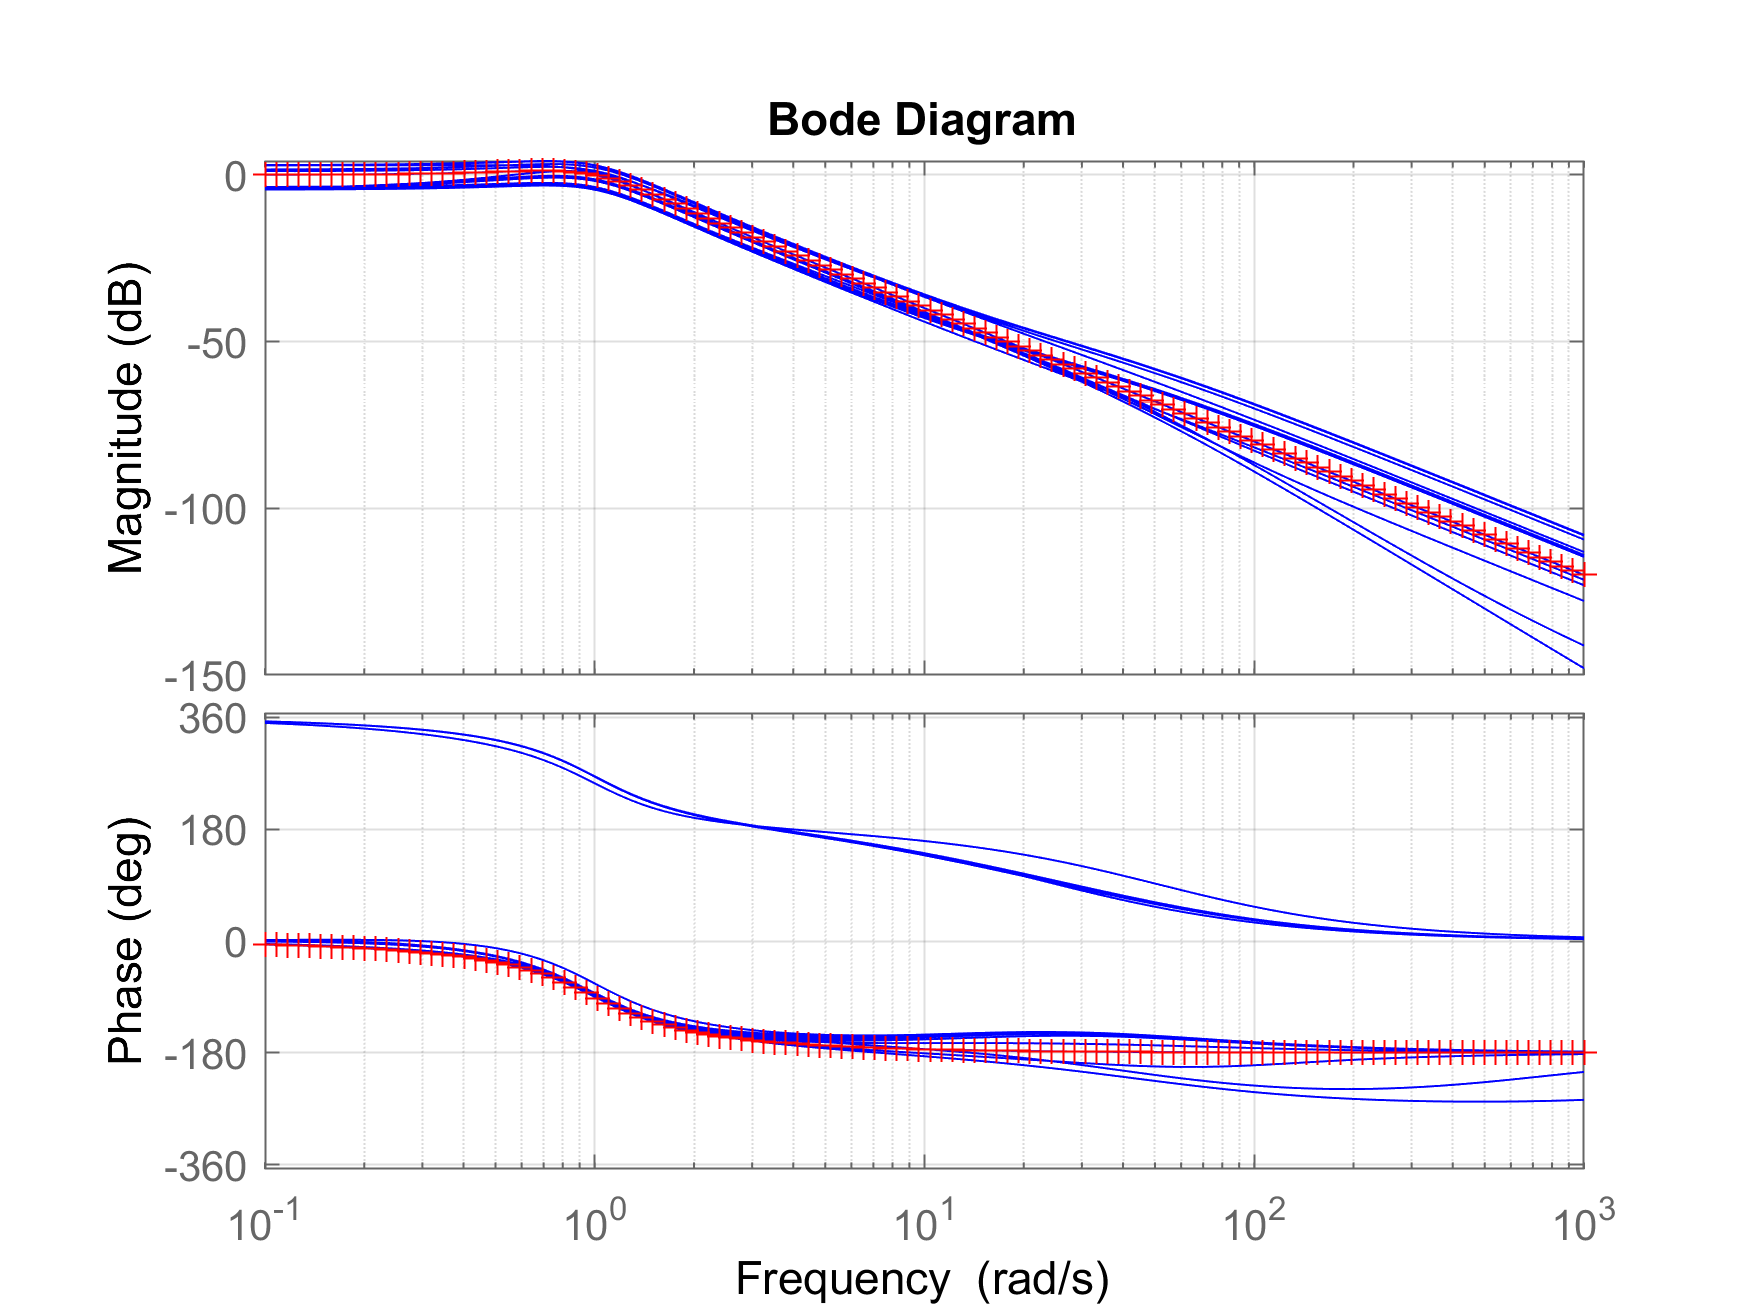
\includegraphics[width=\textwidth]{figures/bode_G.png}
        \caption{}
        \label{fig:bode_G}
    \end{subfigure}
    \begin{subfigure}{0.45\textwidth}
        \centering
        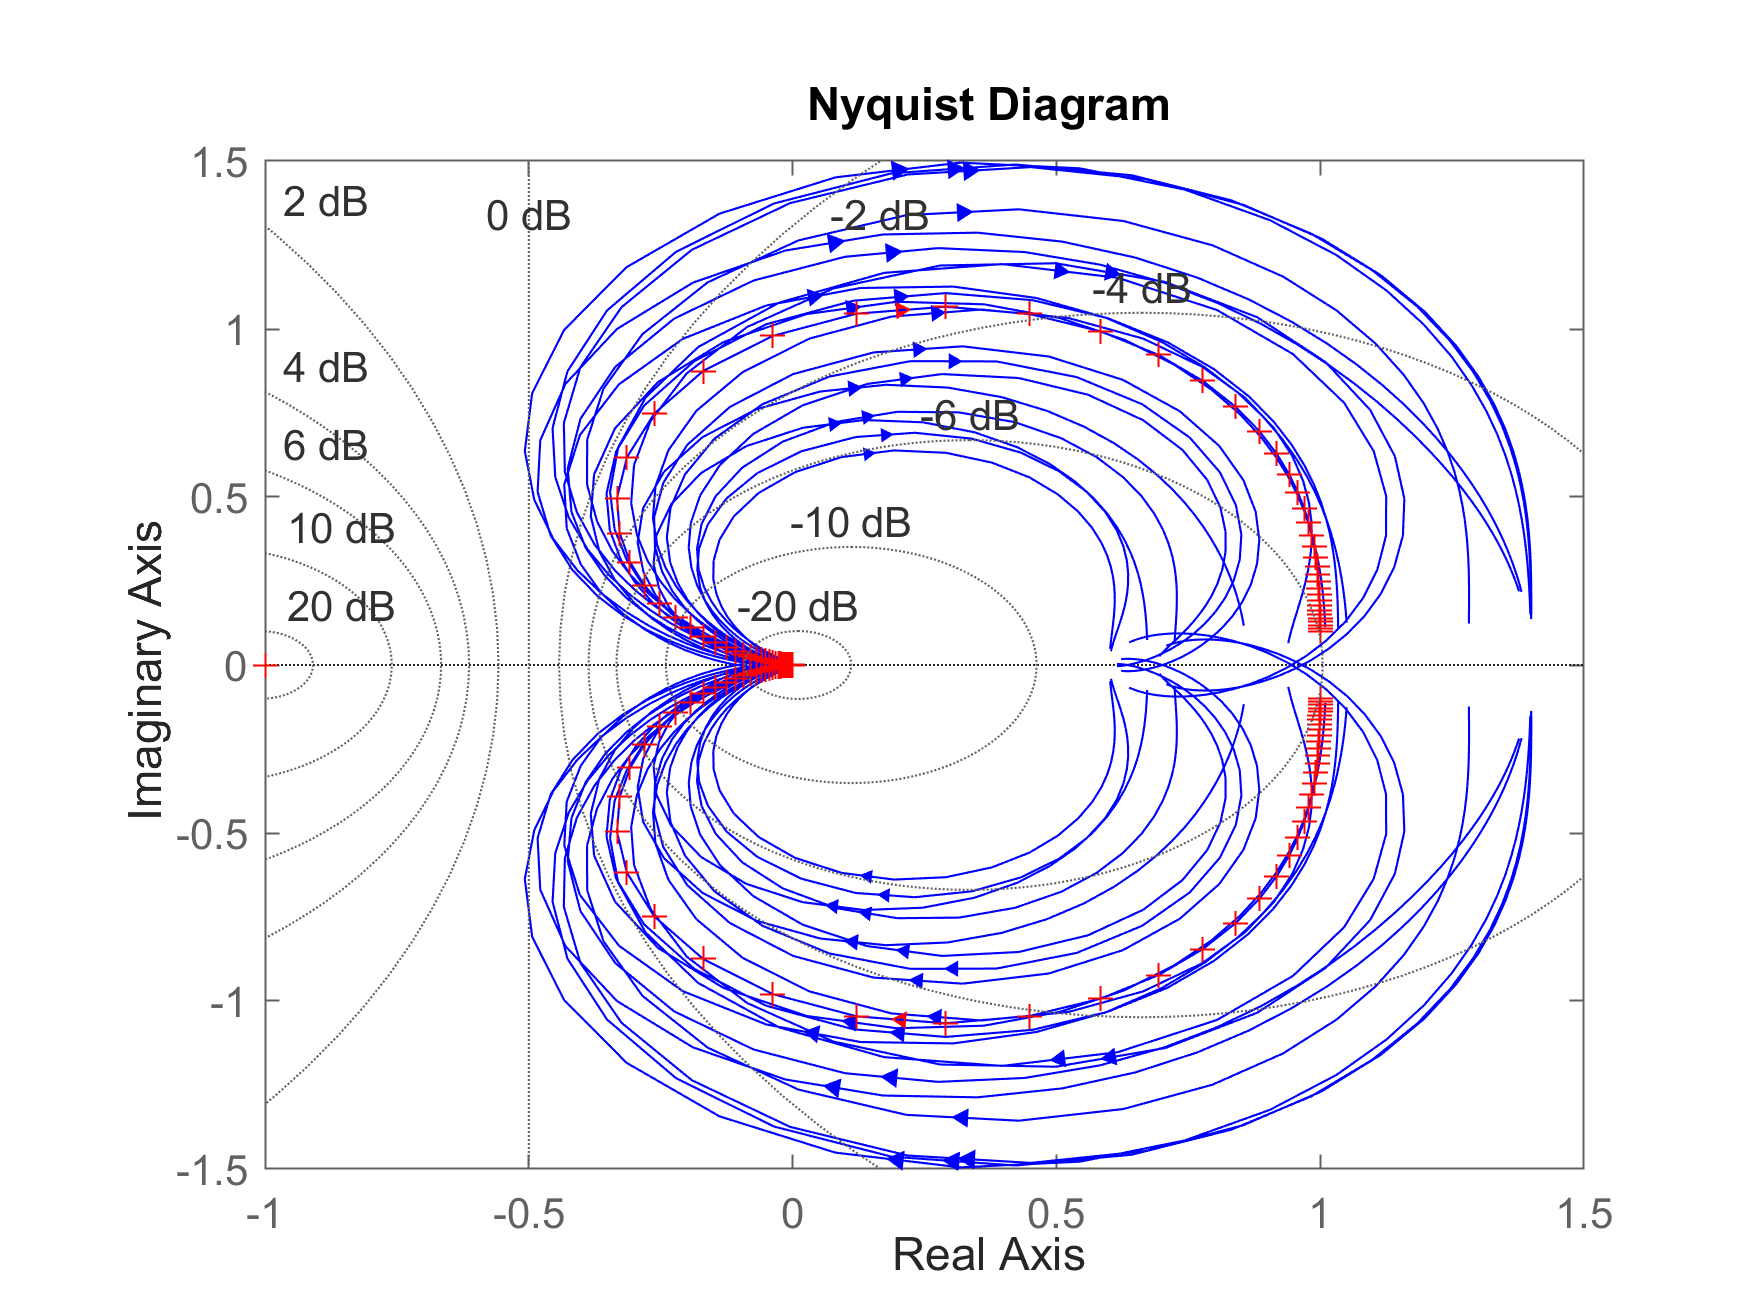
\includegraphics[width=\textwidth]{figures/nyquist_G.png}
        \caption{}
        \label{fig:nyquist_G}
    \end{subfigure}
    \caption{}
\end{figure}


From the Nyquist plot in figure \ref{fig:nyquist_G} the gain margin is infinite and the phase margin is 90 degrees.

\subsection{Tracking performance}


The error transfer function of the closed loop is found by evaluating $E(s) = 1/(1+kG(s))$.
For the steady state error to a step response is found by $\frac{1}{s} \cdot E(s)$ and the final value theorem.
\begin{equation}
    \lim_{t \to \infty} e(t) = \lim_{s \to 0} \left( \frac{s}{s} \cdot \frac{\frac{c_p}{m}s^2 + \frac{c_v}{m}s + \frac{c_p}{m}}{s^2 + \frac{c_v}{m}s + (1+k)\frac{c_p}{m}} \right) = \frac{1}{1+k}
\end{equation}
Therefore as $k \to \infty$, the steady state error goes to zero.
This error is also independent of parameters and so should not be affected by uncertainty.

However the damping ratio and frequency are strongly affected by these parameters.
\begin{equation}
    s = \sigma \pm j\omega = -\frac{c_v}{2m} \pm j \frac{1}{2} \sqrt{4(1+k)\frac{c_p}{m} - \left(\frac{c_v}{m}\right)^2}
\end{equation}
\begin{equation}
    \zeta = \frac{-\sigma }{ \sqrt{\sigma^2 + \omega^2}}
\end{equation}

The poles natural frequency is then shown to increase with k, which decreases the damping ratio.
This is also shown graphically on the root locus plot in figure \ref{fig:rlocus_G}.
As $k$ increases, the poles move away from the real axis and the angle between pole and imaginary axis ($\arcsin(\zeta)$) decreases.

\begin{figure}[H]
    \centering
    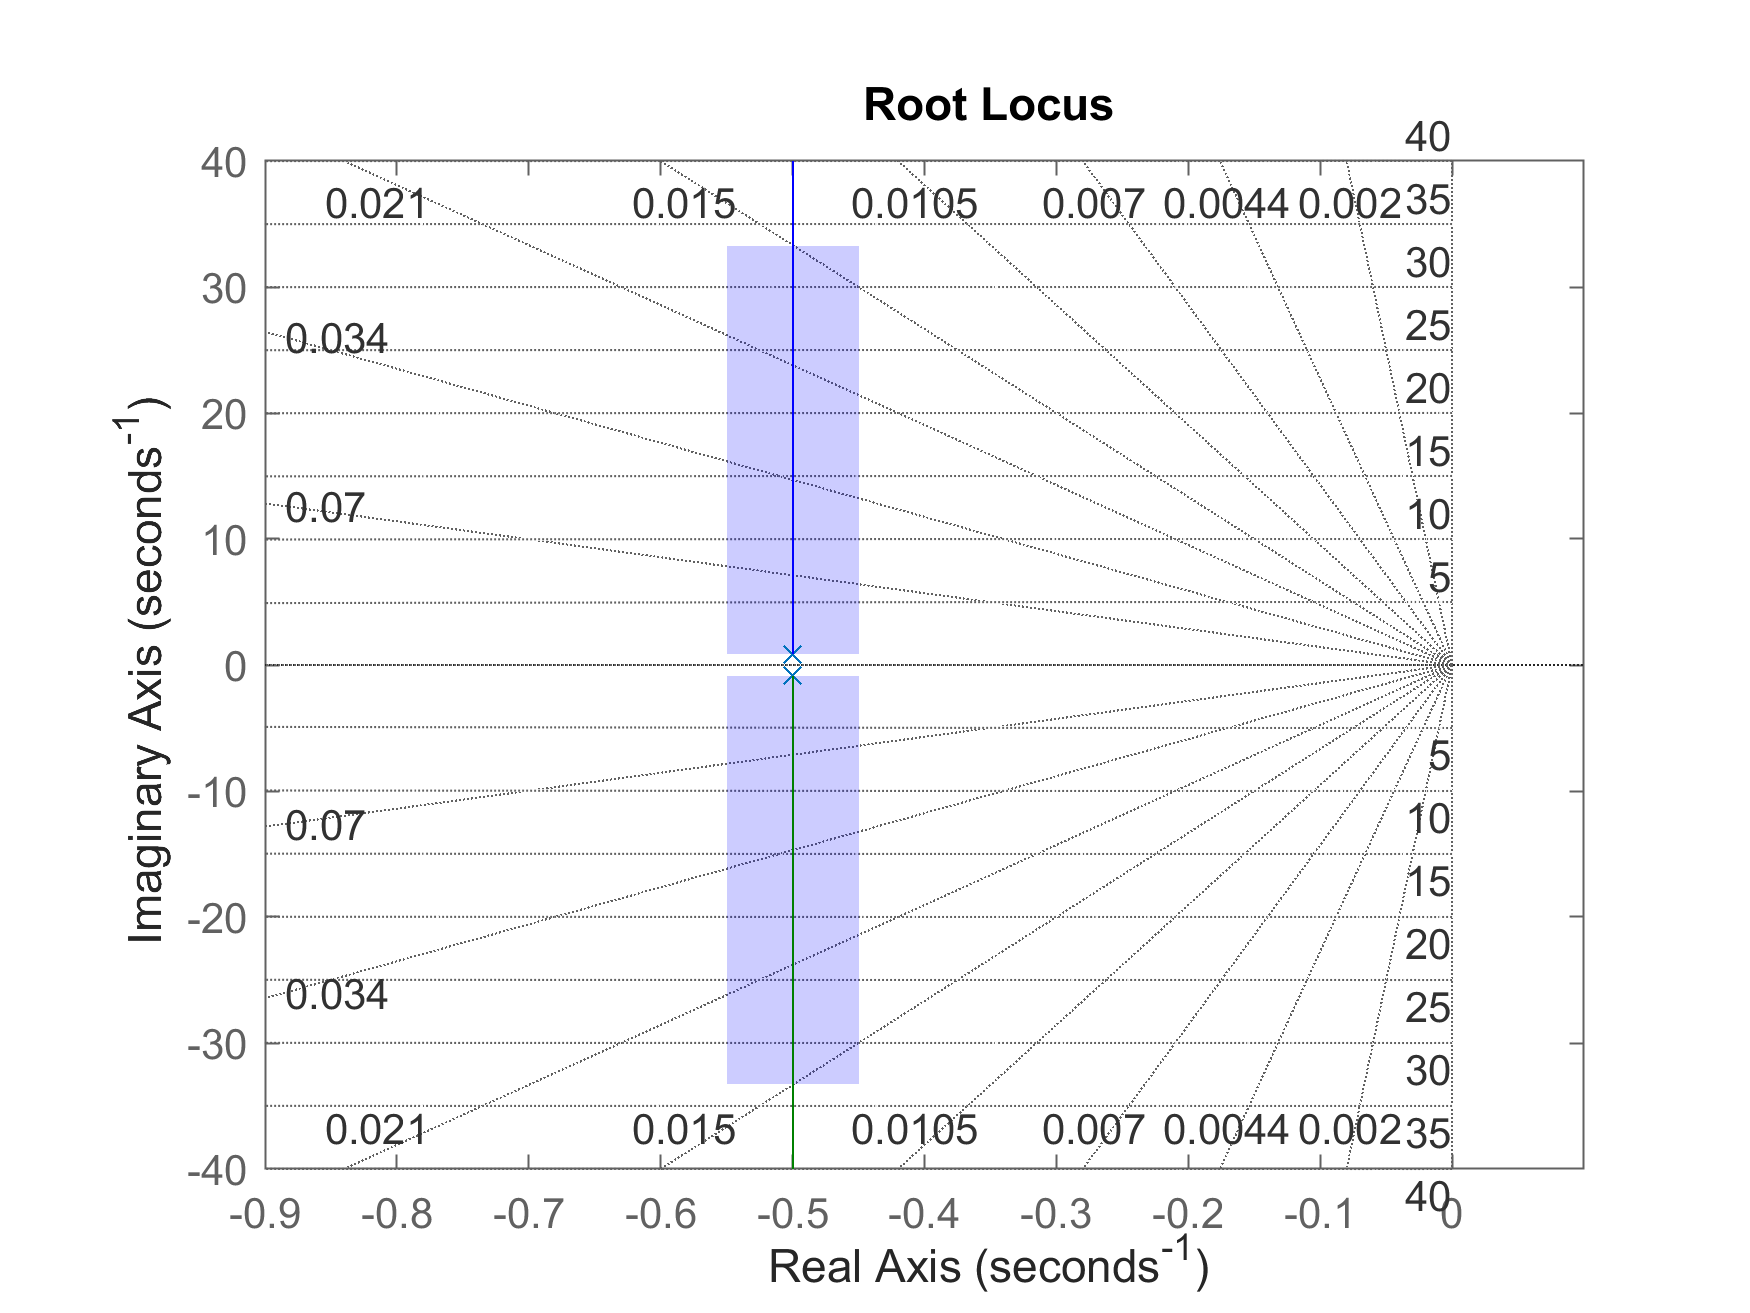
\includegraphics[width=0.6\textwidth]{figures/rlocus_G.png}
    \caption{}
    \label{fig:rlocus_G}
\end{figure}

Figure \ref{fig:rlocus_G} shows the root locus plot for the nominal system for positive values of $k$.
The plot also shows the region of possible pole locations for the parametric uncertainty given in table \ref{tab:parameters}.

\begin{figure}[H]
    \centering
    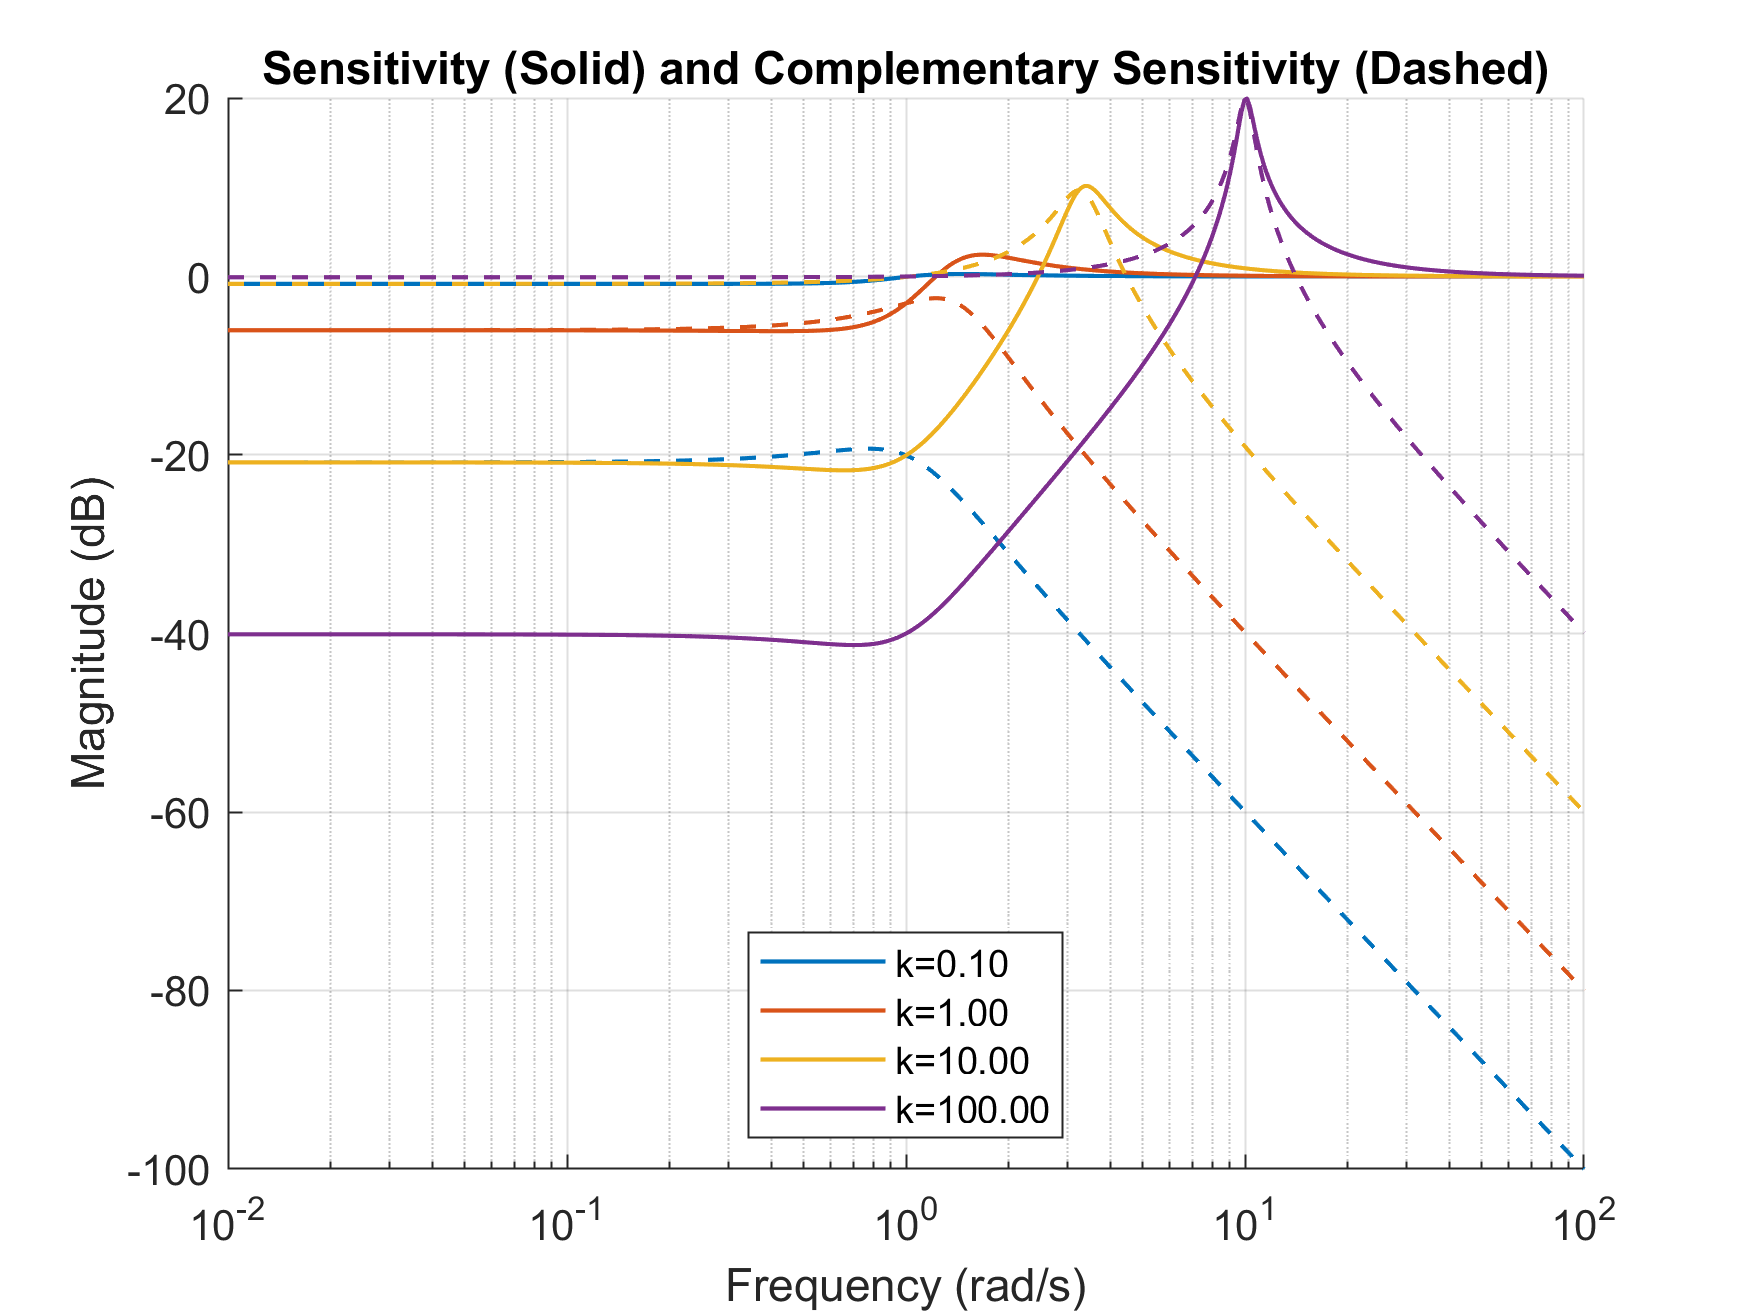
\includegraphics[width=0.6\textwidth]{figures/sensitivities.png}
    \caption{}
    \label{fig:sensitivities}
\end{figure}

Figure \ref{fig:sensitivities} shows the sensitivity and complementary sensitivity response plot for disturbance and reference inputs.
High frequency reference signals are attenuated more by smaller values of $k$. Similarly, high frequency disturbances are amplified less at smaller values of $k$.
At low frequency and small values of k, the sensitivity is higher than the complementary sensitivity which is not desirable.

To gain insight into how parametric uncertainty impacts the system response uncertainty must be propagated as follows:
\begin{equation}
    \delta \omega = \frac{\partial \omega}{\partial c_p} \delta c_p + \frac{\partial \omega}{\partial c_v} \delta c_v \quad \delta \zeta = \frac{\partial \zeta}{\partial c_p} \delta c_p + \frac{\partial \zeta}{\partial c_v} \delta c_v
\end{equation}
The derivatives can be found analytically and are shown plotted against $k$ at otherwise nominal values in figure \ref{fig:u_propagation}.

\begin{figure}[H]
    \centering
    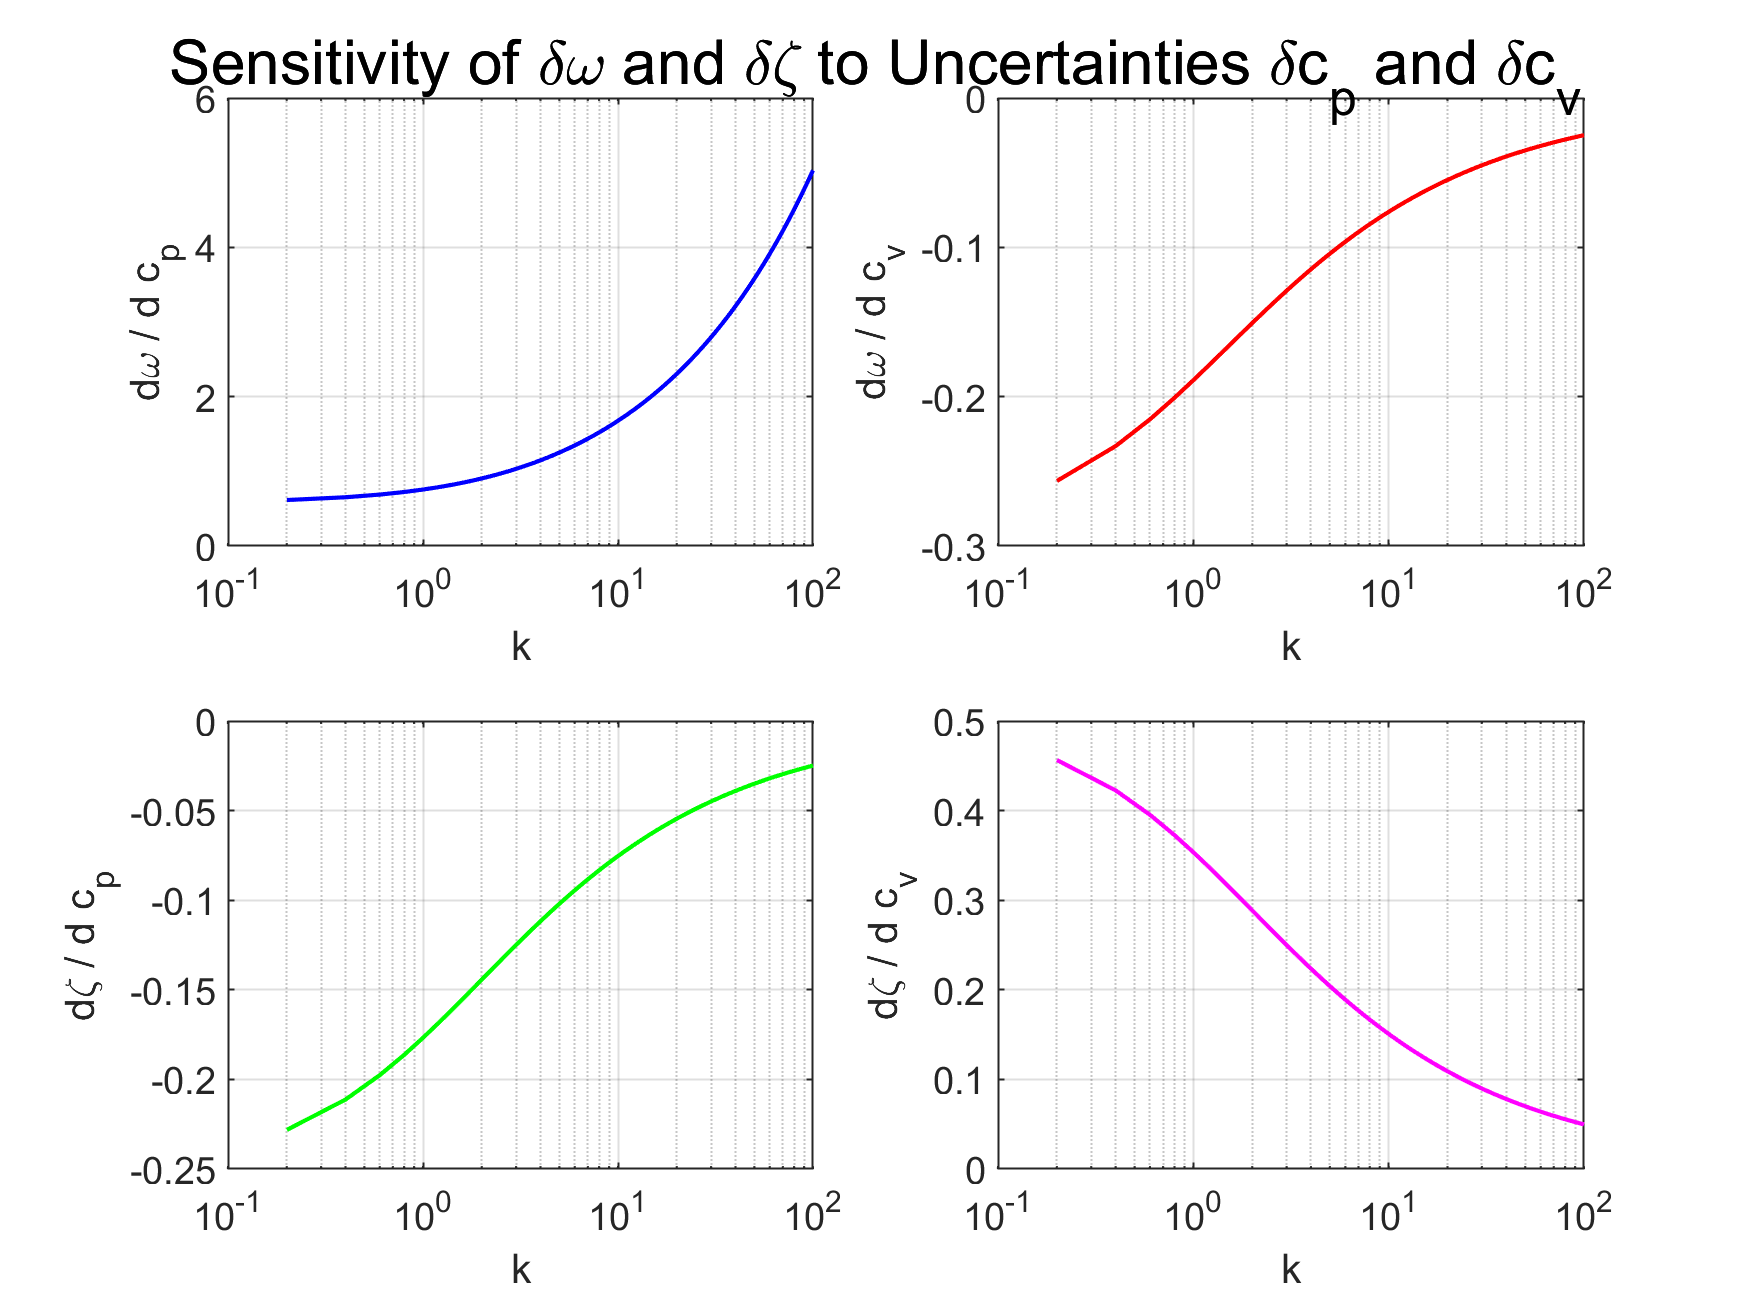
\includegraphics[width=0.6\textwidth]{figures/u_propagation.png}
    \caption{}
    \label{fig:u_propagation}
\end{figure}
Figure \ref{fig:u_propagation} shows how the uncertainty in response parameters changes with $k$.
Small changes in damping ratio due to the parametric uncertainty become less pronounced as $k$ increases.
However, the component of uncertainty in the frequency due to the stiffness coefficient, $c_p$, is shown to increase with $k$.

\subsection{Bound on perturbed plant}

The perturbed plant can be written as $G_p(s) = G(s) + \Delta G(s)$ where $\Delta G(s)$ is the additive perturbation.
This can be rearranged and the perturbed plants parameters can include absolute uncertainty $\Delta_p$ and $\Delta_v$.
\begin{equation}
    \Delta = \frac{s\left(\Delta_p c_v - \Delta_v c_p + \Delta_p m s\right)}
    {\left(m s^2 + c_v s + c_p\right)\left(\Delta_p + c_p + \Delta_v s + c_v s + m s^2\right)}    
    \label{eq:analytical_delta}
\end{equation}
Generally, the maximum value of $\Delta$ for a given frequency could occur at any combination parameter uncertainties.
For this case however, it was found that $\Delta_p = -0.1$ and $\Delta_v = 0.075$ is close to the maximum value of $\Delta$ for a wide range of frequencies.

\begin{figure}[H]
    \centering
    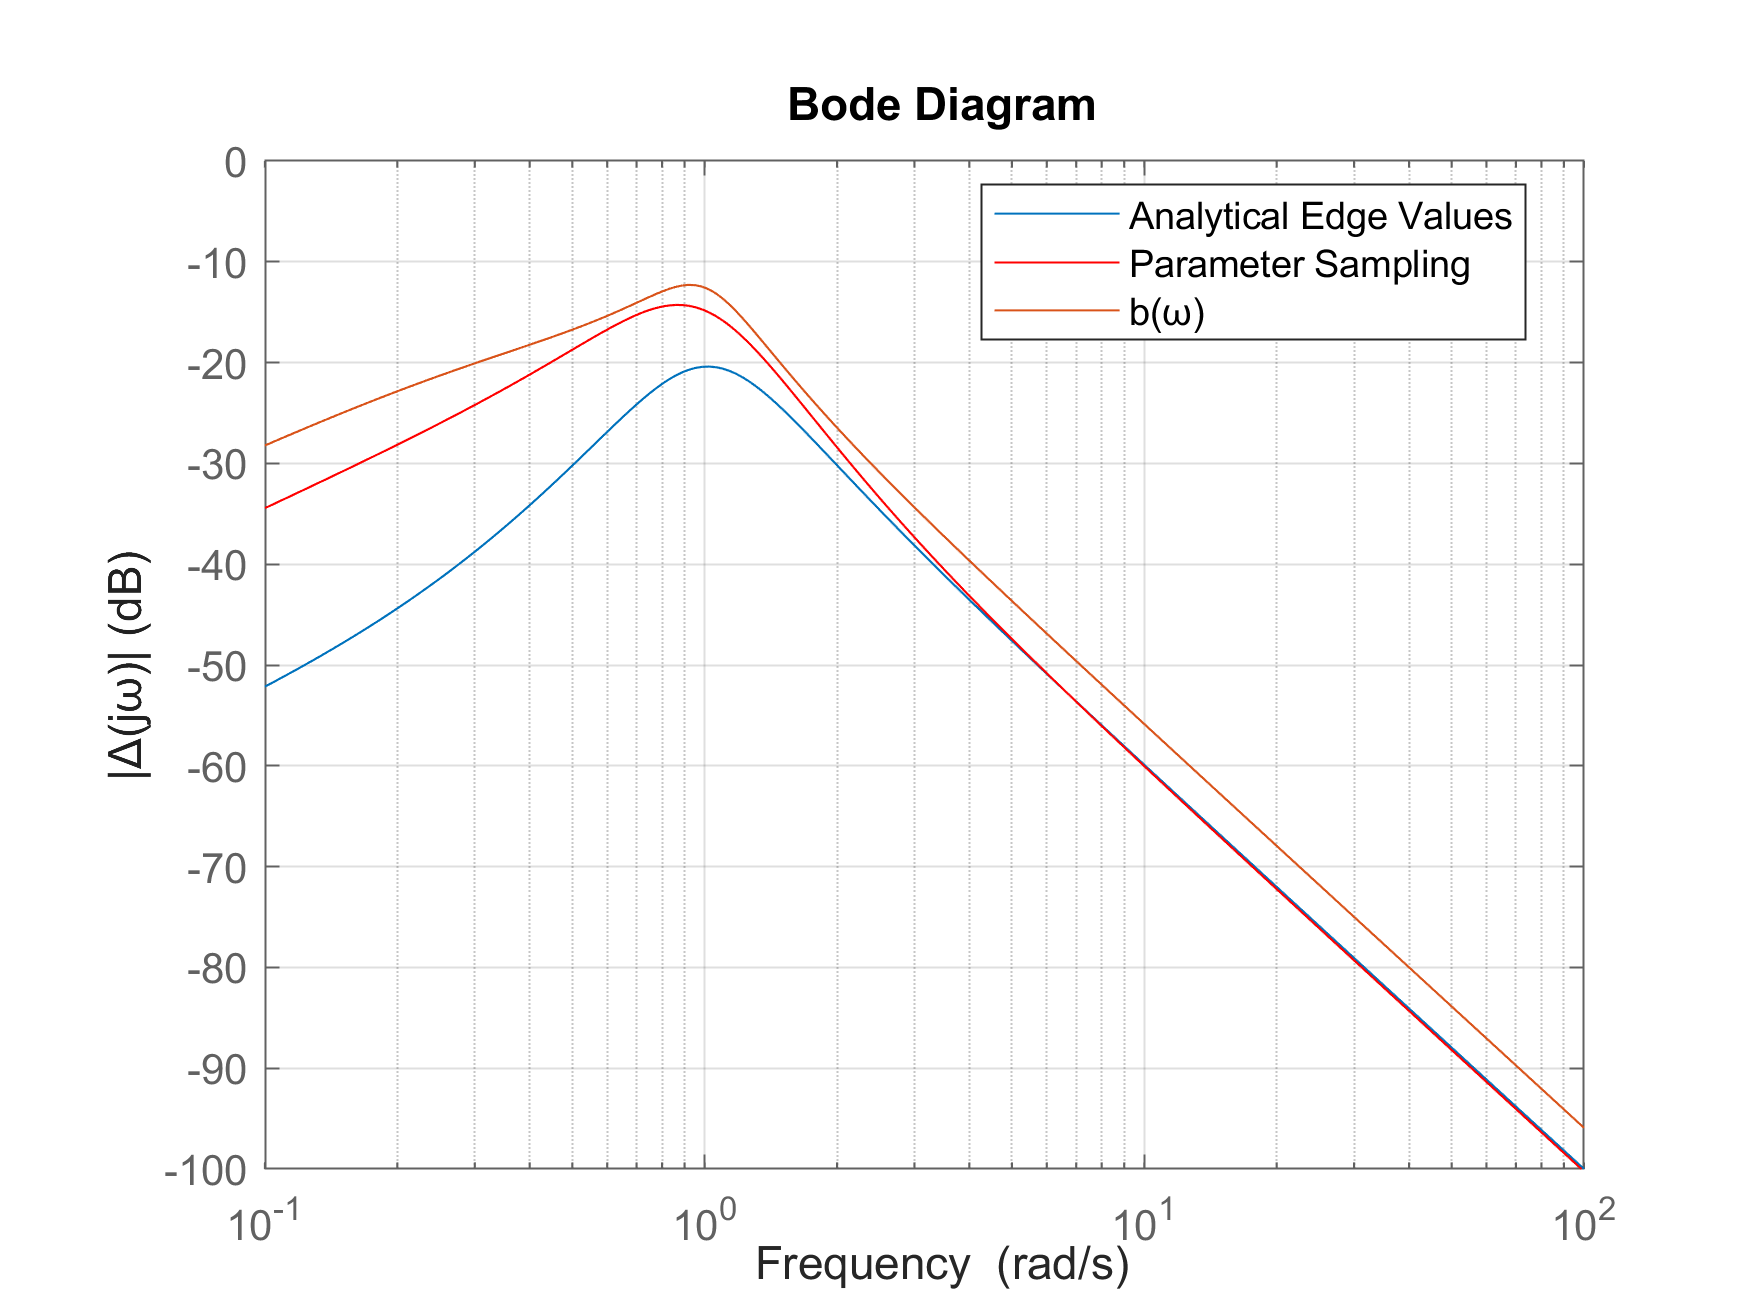
\includegraphics[width=0.6\textwidth]{figures/1_tight_bound.png}
    \caption{}
    \label{fig:bode_Gp}
\end{figure}

Figure \ref{fig:bode_Gp} shows the bode plot of bounds on the additive perturbation from the nominal plant.
The analytical bound is shown as a reference and was found using equation \ref{eq:analytical_delta} with $\Delta_p = 0.1$ and $\Delta_v = 0.075$

It was decided that a very small additional bound would be added above the tight bound to guarantee robustness within the confidence interval in the parameter sampling.
The robustness bound was increased further at lower frequencies, which were felt to be more important in the application of soft robotics.

\begin{equation}
    b(s) = \frac{0.16s^2 + 0.139s}{s^4 + 1.95s^3 + 2.15s^2 + 1.55s + 0.346}
    \label{eq:bound1}
\end{equation}

\subsection{Weight design}

\begin{equation}
    \begin{Vmatrix}
        W_1 S \\
        W_2 KS \\
        W_3 T
    \end{Vmatrix}_\infty \le 1 \implies
    \begin{cases}
        ||S||_\infty \le |1/W_1| \\
        ||KS||_\infty \le |1/W_2| \\
        ||T||_\infty \le |1/W_3|
    \end{cases}
\end{equation}

\subsubsection{Closed loop tracking error below -40dB at frequencies lower than $\omega_1=6\pi$ rad/s \label{pnt:tracking}}

The tracking error from $r$ to $e$ is given by $e = r - y = (1 - KS)r = Sr$. Therefore a weight function $W_1(s)$ of +40dB below the frequency $\omega_1 = 6\pi$ rad/s is required to satisfy \ref{pnt:tracking}.
This was done using the MATLAB command \texttt{makeweight(100, 6*pi, 0.9);}

\subsubsection{robust stability for additive dynamic uncertainties defined by equation \ref{eq:bound1} \label{pnt:robust}}

It isnt known what to do for this

\subsubsection{Disturbance attenuation from sensor noise to ouput of -40dB above the frequency $\omega_2 = 500\pi$ rad/s \label{pnt:disturbance}}

The output y is also affected by sensor noise $y = T(r - d)$ and so a weight function $W_3(s)$ of -40dB above the frequency $\omega_2 = 500\pi$ rad/s is required to satisfy \ref{pnt:disturbance}.

\subsection{Controller Synthesis}

\subsubsection{The $H_\infty$ controller $K_N(s)$ that meets tracking performance and disturbance rejection}

\subsubsection{The $H_\infty$ controller $K_R(s)$ that meets also meets robustness requirements}

\section{Haptic Interface}

\subsection{ $H_\infty$ control design}

\subsubsection{Transfer matrix}

The outputs can be written from the inputs as follows:

\begin{equation}
    \begin{bmatrix}
        y \\
        z \\
    \end{bmatrix} = \begin{bmatrix}
        \bar{f}_H \\
        q_2 \\
        W(s)(q_1 - q_2) \\
        W(s)(\bar{F}_E - \bar{F}_H)
    \end{bmatrix} = G_H(s) \begin{bmatrix}
        q_1 \\
        \bar{f}_E \\
        u_1 \\
        u_2
    \end{bmatrix} = G_H(s) \begin{bmatrix}
        w \\
        u \\
    \end{bmatrix}
\end{equation}

From the equations of motion, the transfer matrix is given by:

\begin{equation}
    G_H(s) = \begin{bmatrix}
        s^2/\alpha & -1/\alpha & -1/\alpha & 0 \\
        1/\alpha & \left(\alpha - \frac{1}{\alpha}\right)/s^2 & - 1/(s^2 \alpha) & 1/s^2 \\
        W\left(1 - 1/\alpha \right) & - W\left( \alpha- 1/\alpha \right)/s^2 & W / (s^2 \alpha) & - W/s^2 \\
        W s^2 / \alpha & W(1 - 1/\alpha) & - W/\alpha & 0 \\
    \end{bmatrix}
\end{equation}
Where $\alpha = (\tau s + 1)^2$ and $\tau = 0.05$.

\subsubsection{Linear Matrix Inequalities (LMIs) for bounded gain}

To obtain the LMIs the system is first restacked into \texttt{[z; y]}, a format preferred by MATLAB.
Then from the equations below
\begin{equation}
    \begin{bmatrix}
        z \\
        y
    \end{bmatrix} = \begin{bmatrix}
        Cz \\
        Cy
    \end{bmatrix} x + \begin{bmatrix}
        D_{zw} & D_{zu} \\
        D_{yw} & D_{yu}
    \end{bmatrix} \begin{bmatrix}
        w \\
        u
    \end{bmatrix} \quad \text{and} \quad \dot{x} = Ax + \begin{bmatrix}
        B_w & B_u \\
    \end{bmatrix} \begin{bmatrix}
        w \\
        u
    \end{bmatrix}
\end{equation}

The LMIs shown in fig \ref{fig:bounded_lmi} were used to find a controller with the gain from $w$ to $z$ constrained to be less than 0.1.
%you may want to relax the weighting function W (s) in a reasoned way to achieve feasibility (explain your choice)
The fourth order low pass weighting function was found to achieve a feasible solution without being relaxed.

\begin{figure}[H]
    \centering
    \begin{subfigure}{0.45\textwidth}
        \centering
        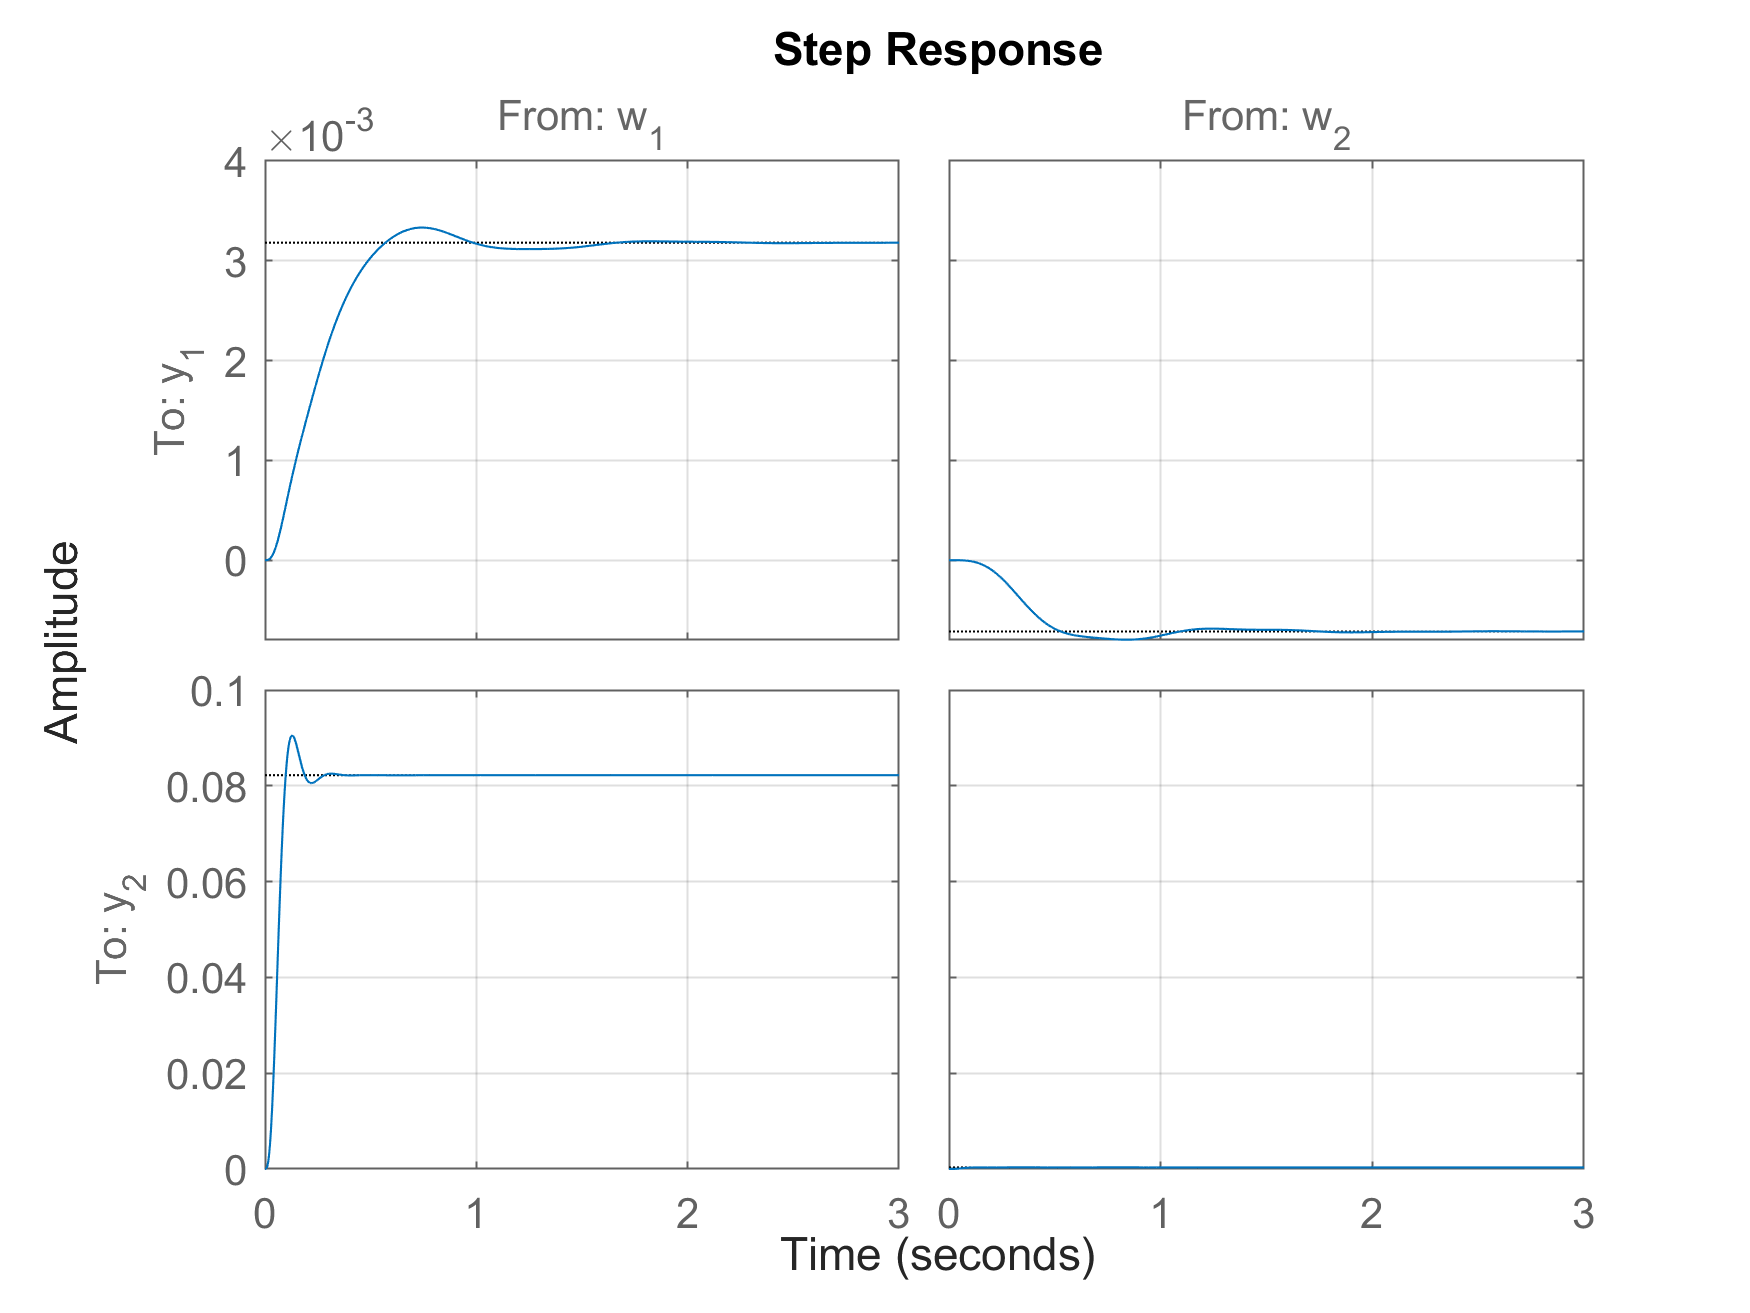
\includegraphics[width=\textwidth]{figures/K_g_step.png}
        \caption{}
    \end{subfigure}    
    \begin{subfigure}{0.45\textwidth}
        \centering
        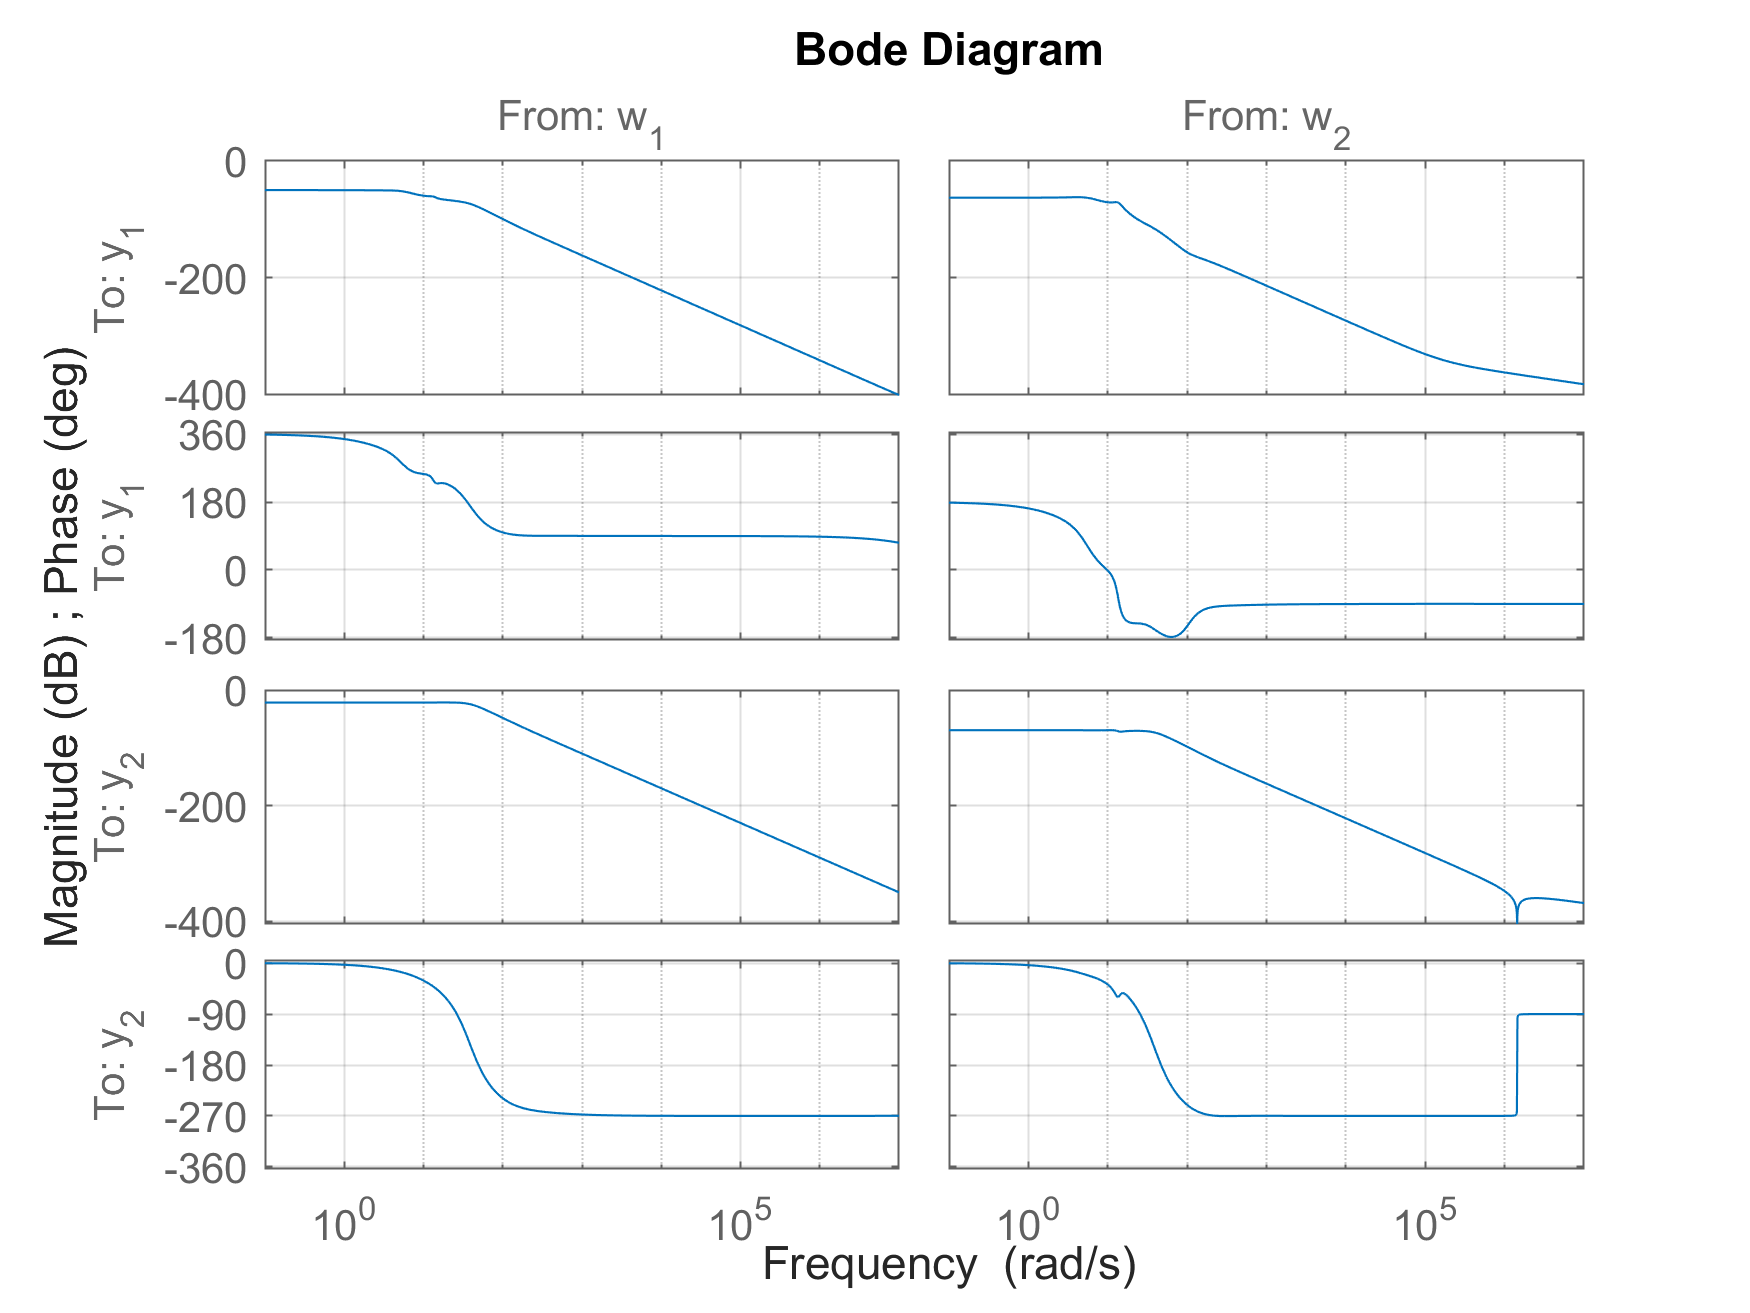
\includegraphics[width=\textwidth]{figures/K_g_bode.png}
        \caption{}
    \end{subfigure}
\end{figure}

\subsubsection{Uncertain feedback}

\begin{figure}[H]
    \centering
    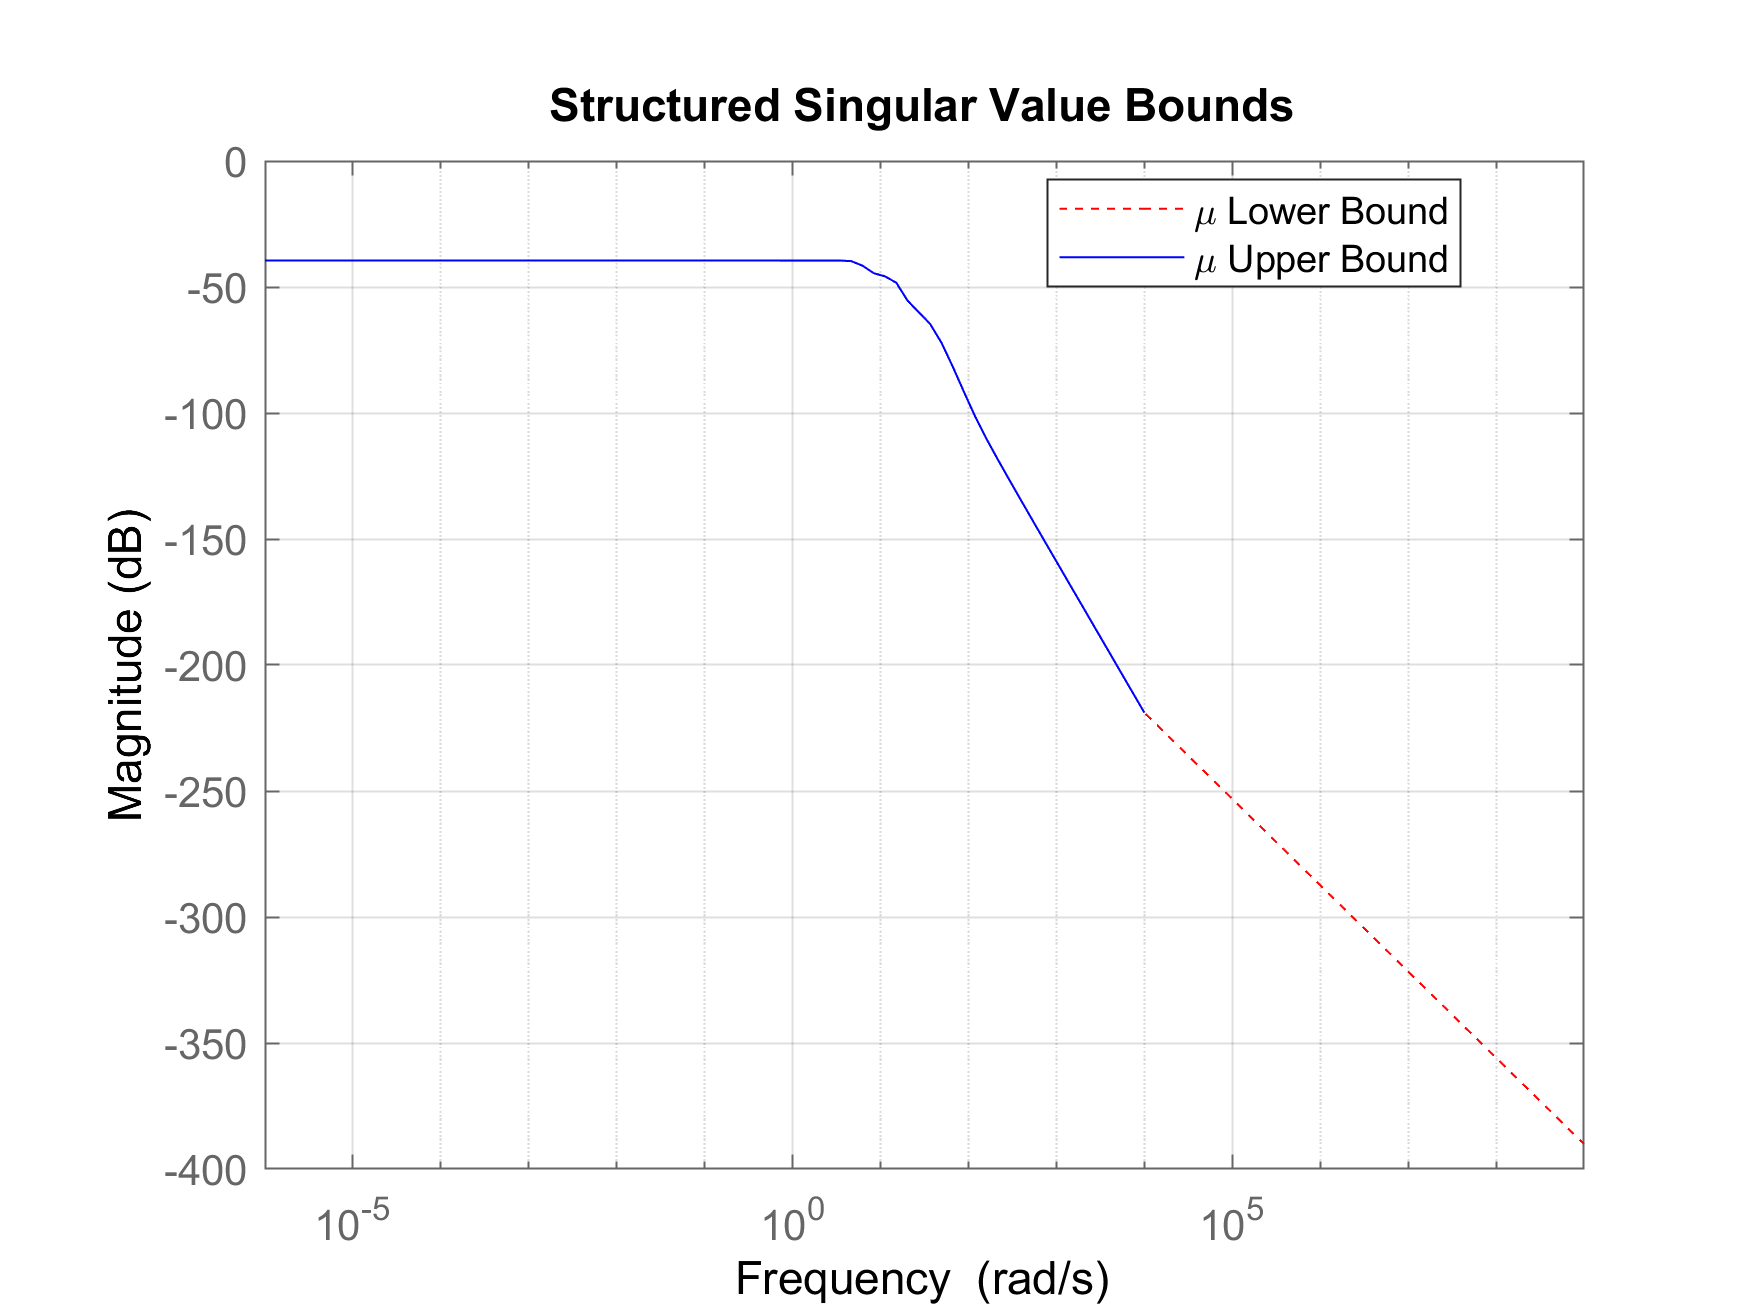
\includegraphics[width=0.6\textwidth]{figures/structured_singular_values.png}
    \caption{}
    \label{fig:structured_singular_values}
\end{figure}

Figure \ref{fig:structured_singular_values} shows the \textit{structured singular value} for the uncertain feedback system.
This \textit{structured singular value} $\mu$ is the smallest $\gamma$ for which this stability condition holds \cite{matlab_robustmu}.
$1/\mu$ is the largest uncertainty level $1/\gamma$ for which the system of uncertain feedback is stable.


\subsection{Passivity-based design}

For the passive arrangement the inputs and outputs are given by:

\begin{equation}
    \begin{bmatrix}
        y \\
        z
    \end{bmatrix} = \begin{bmatrix}
        \dot{q}_1 \\
        \dot{q}_2 \\
        q_1 - q_2 \\
        \dot{q}_1 - \dot{q}_2
    \end{bmatrix} = G_P(s) \begin{bmatrix}
        f_H \\
        f_E \\
        u_1 \\
        u_2
    \end{bmatrix} = G_P(s) \begin{bmatrix}
        w \\
        u
    \end{bmatrix}
\end{equation}

The transfer matrix is given by:
\begin{equation}
    G_P = 
    \begin{bmatrix}
        0 & \frac{1}{\alpha} & 0 & 0 \\[6pt]
        0 & \frac{1}{\alpha} & 0 & \frac{1}{\alpha} \\[6pt]
        \frac{\beta}{s^2} & -\frac{\beta}{s^2} & \frac{1}{s^2} & -\frac{1}{s^2} \\[6pt]
        \frac{\beta}{s} & -\frac{\beta}{s} & \frac{1}{s} & -\frac{1}{s}
    \end{bmatrix}
\end{equation}
Where $\alpha = (\tau s + 1)^2$ as before and $\beta = 1 - 1/\alpha$.

\subsubsection{Transfer matrix for passive arrangement} 

\subsubsection{LMIs for passivity and bounded gain}

\begin{figure}[H]
    \centering
    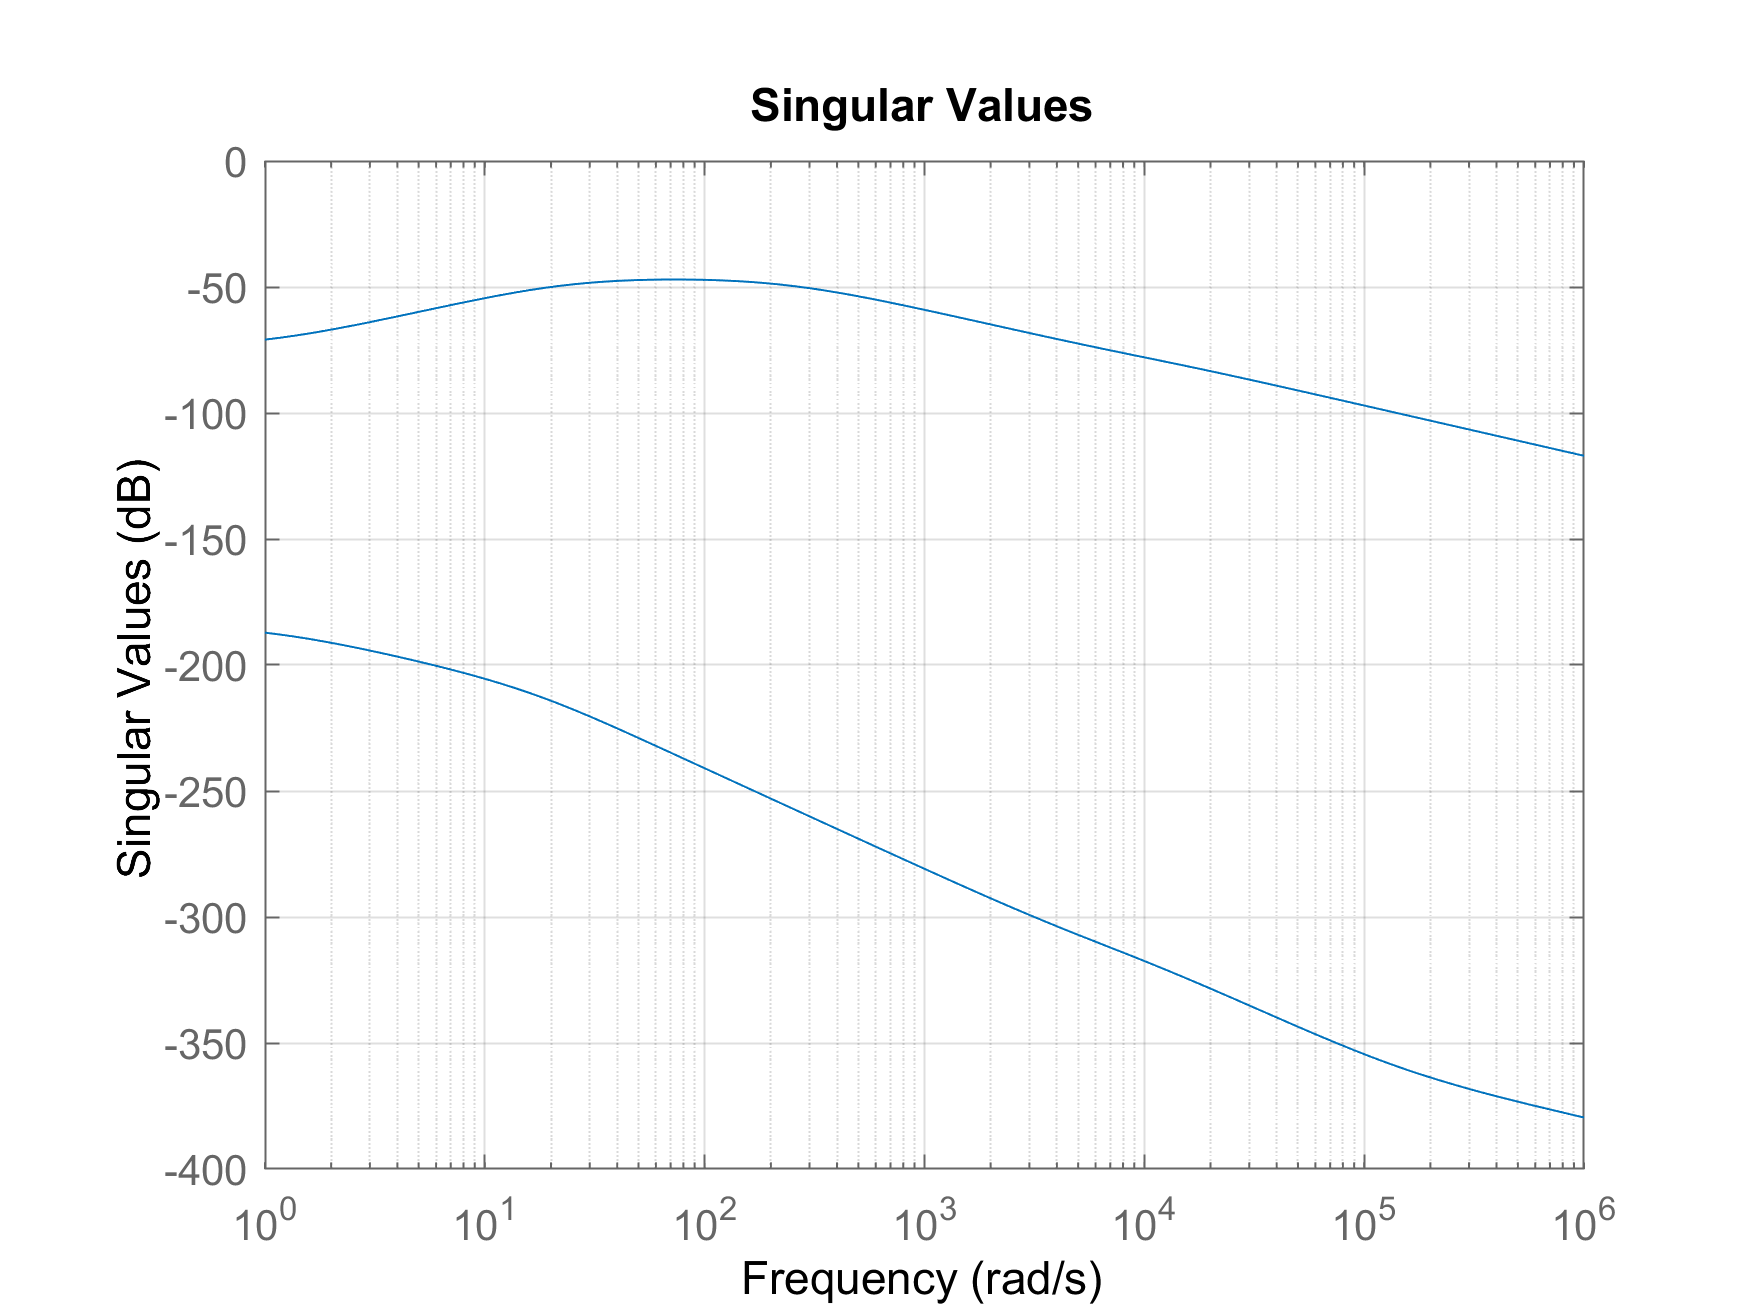
\includegraphics[width=0.6\textwidth]{figures/K_p_sigma.png}
    \caption{}
\end{figure}

\begin{figure}[H]
    \centering
    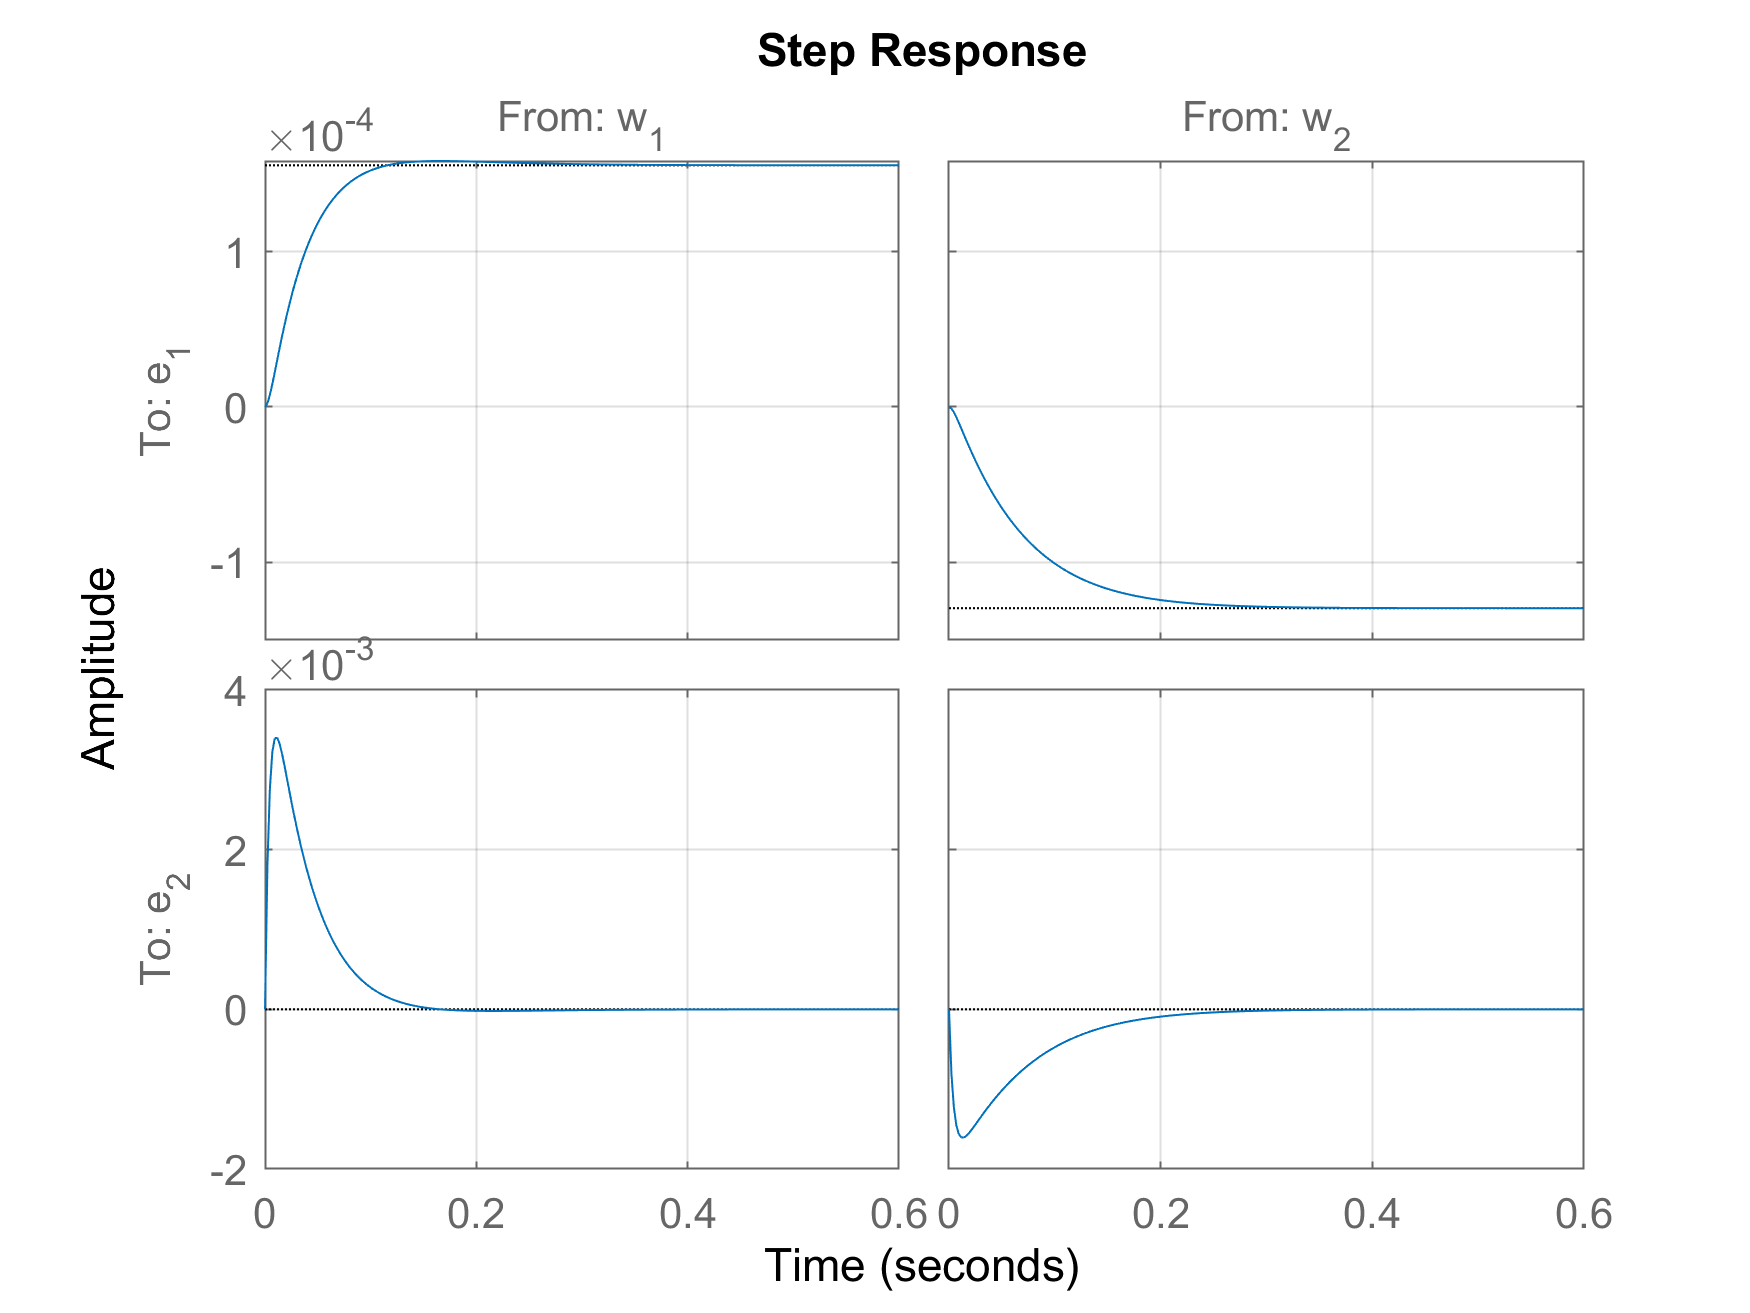
\includegraphics[width=0.6\textwidth]{figures/K_p_step.png}
    \caption{}
\end{figure}

\subsection{Comparison $H_\infty$ and passivity-based control}

% choose simulation!!!

\section{Appendix}


\begin{figure}[H]
    \centering
    \begin{lstlisting}
        cvx_begin sdp
            variable Y(n,n) symmetric
            variable Z(m,n)
            variable gama

            LMI1 = Y >= 0
            LMI2 = gama <= 0.1
            
            LMI3 = [ (Y*A' + A*Y + Z'*Bu' + Bu*Z),   (Y*C' + Z'*D_u'),          Bw;
                    (C*Y + D_u*Z),  -gama*eye(2),      D_w';
                    Bw',            D_w,                -gama*eye(2) ] <= 0;
        cvx_end
    \end{lstlisting}
    \caption{CVX code for bounded gain controller}
    \label{fig:bounded_lmi}
\end{figure}

\begin{figure}[H]
    \centering
    \begin{lstlisting}
        cvx_begin sdp
            variable Y(n,n) symmetric
            variable Z(m,n)
            variable epsilon
            variable gama
            
            %minimise(gama)
            minimise(epsilon) % otherwise makes very high

            LMI1 = Y >= 0
            LMI2 = gama <= 0.1
            
            % gain LMI
            %
            LMI3 = [ (Y*A' + A*Y + Z'*Bu' + Bu*Z),   (Y*Cz' + Z'*Dzu'),          Bw;
                    (Cz*Y + Dzu*Z),  -gama*eye(2),      Dzw';
                    Bw',            Dzw,                -gama*eye(2) ] <= 0;
            
            LMI4 = epsilon >= 0
            LMI5 = [ Y*A' + A*Y + Bu*Z + Z'*Bu', Bw - Y*Cy' - Z'*Dyu';
                    Bw' - Cy*Y-Dyu*Z,   -2*epsilon*eye(2) - (Dyw + Dyw')] <= 0
                
        cvx_end
    \end{lstlisting}
    \caption{CVX code for bounded gain and passivity controller}
    \label{fig:bounded_passive_lmi}
\end{figure}

\begin{thebibliography}{9}

    %Endres, SC, Sandrock, C, Focke, WW (2018) “A simplicial homology algorithm for lipschitz optimisation”, Journal of Global Optimization.
    
      \bibitem{handout}
      F. Forni, R, Sepulchre
      \emph{4F2, Robust and Nonlinear Control: Coursework 1}
      University of Cambridge,
      2025.
    
      \bibitem{matlab_robustmu}
      MATLAB
      \emph{Robust Performance Measure for Mu Synthesis}
      \texttt{https://uk.mathworks.com/help/robust/ug/measures-of-robust-performance.html}

    
\end{thebibliography}

\end{document}